\documentclass[border=2pt]{standalone}
\usepackage{tikz}
\usetikzlibrary{patterns}
\begin{document}
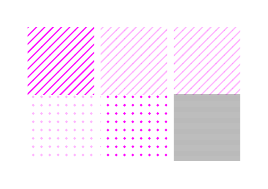
\begin{tikzpicture}[x=24pt,y=24pt,pattern color=magenta]
  \fill[pattern=north east lines,fill opacity=.3] (0,1) rectangle (1,2);
  \fill[pattern=north east lines,draw opacity=.3] (1.1,1) rectangle (2.1,2);
  \fill[pattern=north east lines,opacity=.3] (2.2,1) rectangle (3.2,2);
  \fill[pattern=dots,fill opacity=.3] (0,0) rectangle (1,1);
  \fill[pattern=dots,draw opacity=.3] (1.1,0) rectangle (2.1,1);
  \fill[pattern=horizontal lines dark gray,fill opacity=.3] (2.2,0) rectangle (3.2,1);
\end{tikzpicture}
\end{document}
